% Chapter 'Evaluation'
In this chapter we will evaluate the performance of our transcription system. bla bla

\section{Methods}

	\subsection{Training and Test Sets}
		The dataset consists of sound segments, segmented based on the annotations. This means that our segmentation of sound (present in our application), will not be part of the evaluation.
		The training and test sets of sounds for the KNN classifier are randomly chosen from the same pool (the dataset). It is distributed between the training and test set in a 70\%/30\% ratio, accordingly, for each class. This means there will not be a fixed number of sounds for each class (neither total nor divided), but rather a fixed distribution between the number of training and test sounds for each class. We can do this instead of e.g. k-fold cross validation, due to scale of our collected dataset. The ratio was suggested by our supervisor\footnote{Bob L. Sturm}. The composition of the entire dataset has been summarized in table \ref{table:eval:datasetComposition}. 
		Furthermore, all sounds with a duration less than the windowsize used for feature calculation, are removed before testing. This is done before splitting the dataset, such as to make sure we do not distort the 70/30 distribution.

		\begin{table}
			\centering
			\begin{tabular}{|l|r|r|}
				\hline
				Value  &  Count  & Percent \\ \hline
		      noise    &  150    & 10.19\% \\ \hline
		          k    &  466    & 31.66\% \\ \hline
		  undefined    &  130    &  8.83\% \\ \hline
		          s    &  331    & 22.49\% \\ \hline
		         hh    &  395    & 26.83\% \\ \hline
		      TOTAL    &  1472	 & 100.00\% \\ \hline

			\end{tabular}
			\caption{Dataset composition}
			\label{table:eval:datasetComposition}
		\end{table}


	\subsection{Variables}
		As the number of combinations of features, and parameters of features and classifiers, is very large, we purposely keep as few variables and as many constants as possible. We chose not to test combinations of features, but rather single features one at a time.
		The primary variable to be tested is the K in the KNN classifier (how many neighbors it considers). Some changes will be made to feature parameters. Each feature will be tested with a couple of different sets of parameters:
		
		\begin{itemize}
			\item MFCC
				\begin{itemize}
					\item 20ms windows, 10ms skip
					\item 10ms windows, 5ms skip
					\item 5ms windows, 2ms skip
				\end{itemize}
			
			\item RMS
				\begin{itemize}
					\item has no parameters, so only 1 test
				\end{itemize}
				
			\item ZCR
				\begin{itemize}
					\item has no parameters, so only 1 test
				\end{itemize}
		
		\end{itemize}
		
		All features will be calculated for $K \in [1;10]$.


	\subsection{Measures}
		A confusion table is created for each test (each unique combination of variables). This will be shown in percentages (or rather, values between 0 and 1). Overall accuracy is calculated, along with precision, recall, and F-score for each class individually. For the sake of compactness, all the measures are included in an extended confusion table, as shown in the explanatory table \ref{table:eval:explanatory}. 
		The most important measure, for the sake of measuring our transcription system, would be the precision, that is, the amount of correctly transcribed sounds over the actual amount of that sound class.
		Recall should just be ignored, since we only test on the dataset, which means that we always test on all available samples of any given class, meaning that it would be the same as the amount of . This would be different, had the segmentation been part of the evaluation. It is included nonetheless, as further progress with this project might find a need for it.

			\begin{table}
				\centering
				\begin{tabular}{|c | c | c | c | c |}
					\hline
					 & Real Class(1) & Real Class(2) & Real Class(3) & Precision\\ \hline
					Label(1)  & ... & ... & ... & ...\\ \hline
					Label(2)  & ... & ... & ... & ...\\ \hline
					Label(3) & ... & ... & ... & ...\\ \hline
					Recall   & ... & ... & ... & \multicolumn{1}{c}{Overall}\\ \cline{1-4}
					F-Score & ... & ... & ... & \multicolumn{1}{c}{Accuracy} \\ \cline{1-4}
				\end{tabular}
				\caption{$K=1$}
				\label{table:eval:explanatory}
			\end{table}
		chi squared?
		sign test?
		
		
	\subsection{Test Implementation}		% REFERENCES TO APPENDIX!
		To ease the testing of the transcription system, two additional scripts were created: testTables.m and testPlots.m.
		The testTables.m script simply runs a test and formats the results in tables usable for \LaTeX, while testPlots.m creates plots for precision, recall, and F over K, including the overall accuracy in all three plots, and saves them as EPS images\footnote{Encapsulated Postscript format - it keeps plots from Matlab sharp and pretty when imported in \LaTeX}. Both scripts are relatively simple and well-commented, and thus should require no more than than a simple mention, as they do not include features not already explained in chapter \ref{chapter:OurApproach}.
			
 
\section{Results}
For all results found, some interpretation of the data and statistics will be presented. Further discussion about the relevance of the data, possible mistakes that affected results, or similar, will be covered in chapter \ref{chapter:Discussion}. 
Confusion tables take up a lot of pages, so any tables not directly relevant can be found in appendix \ref{APPENDIXBORWHATEVER}.


	\subsection{MFCC}
				\begin{figure}
			\begin{minipage}{\textwidth}
				\centering
				\subcaptionbox{Precision}{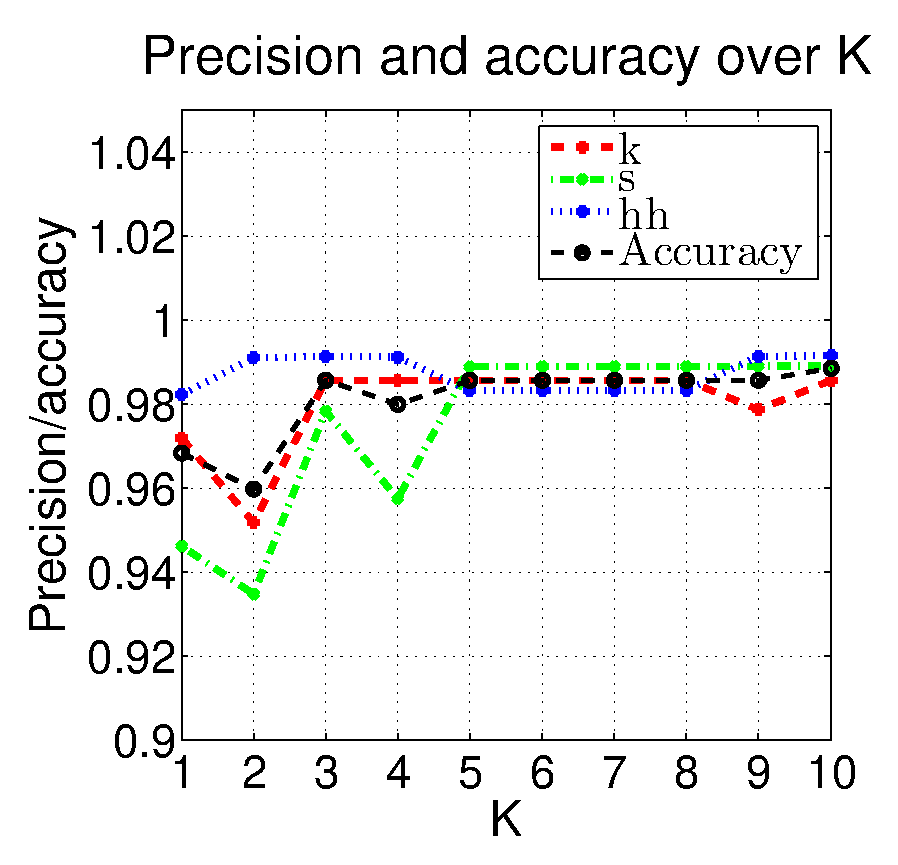
\includegraphics[width=.31\linewidth]{testMFCC20ms10msPrec.eps}}\quad
				\subcaptionbox{Recall}{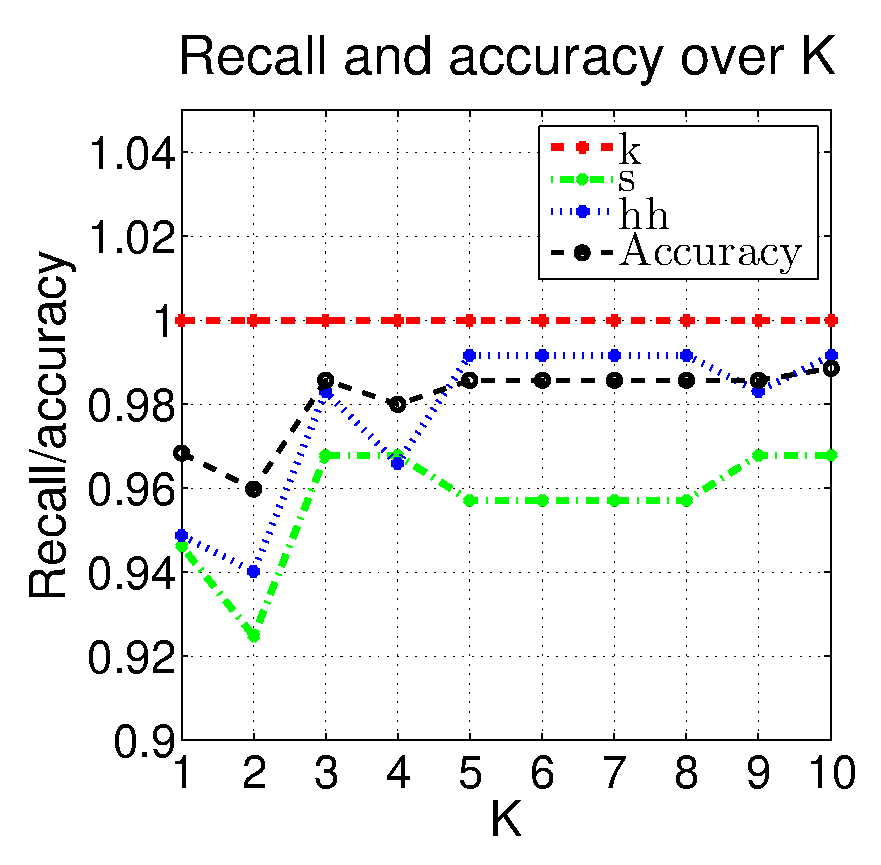
\includegraphics[width=.31\linewidth]{testMFCC20ms10msRec.eps}}\quad
				\subcaptionbox{F}{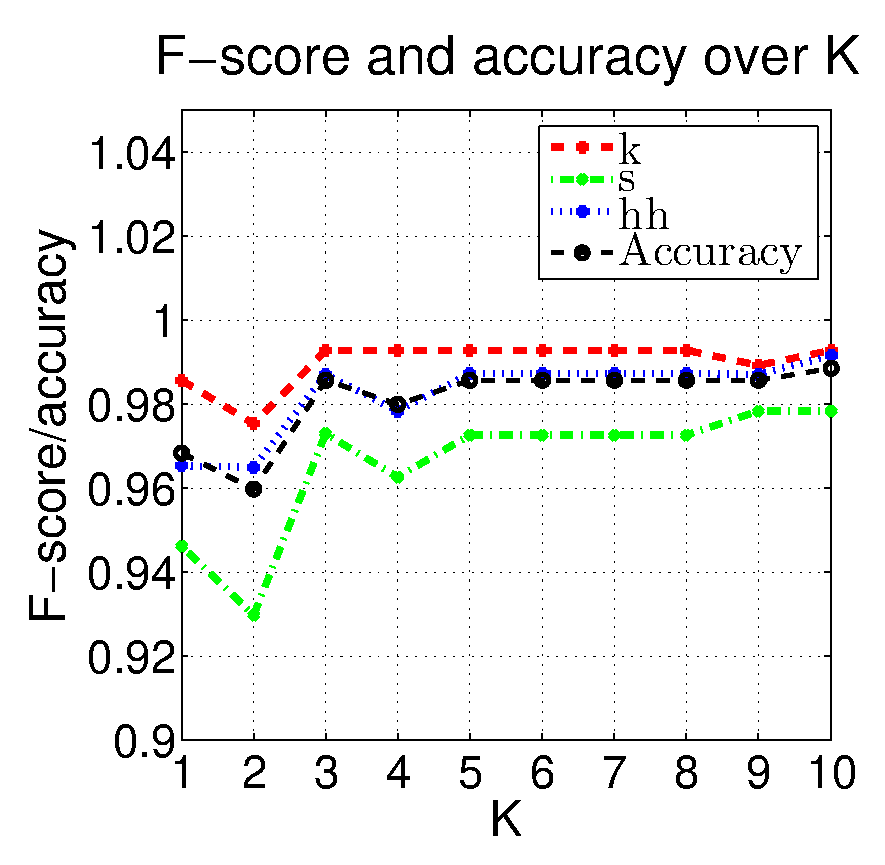
\includegraphics[width=.31\linewidth]{testMFCC20ms10msF.eps}}\quad
				\caption{Result plots for MFCC with 20ms window size and 10ms window skip.}
				\label{fig:eval:testPlotMFCC20ms10ms}
			\end{minipage}\hfill
			
			\begin{minipage}{\textwidth}
				\centering
				\subcaptionbox{Precision}{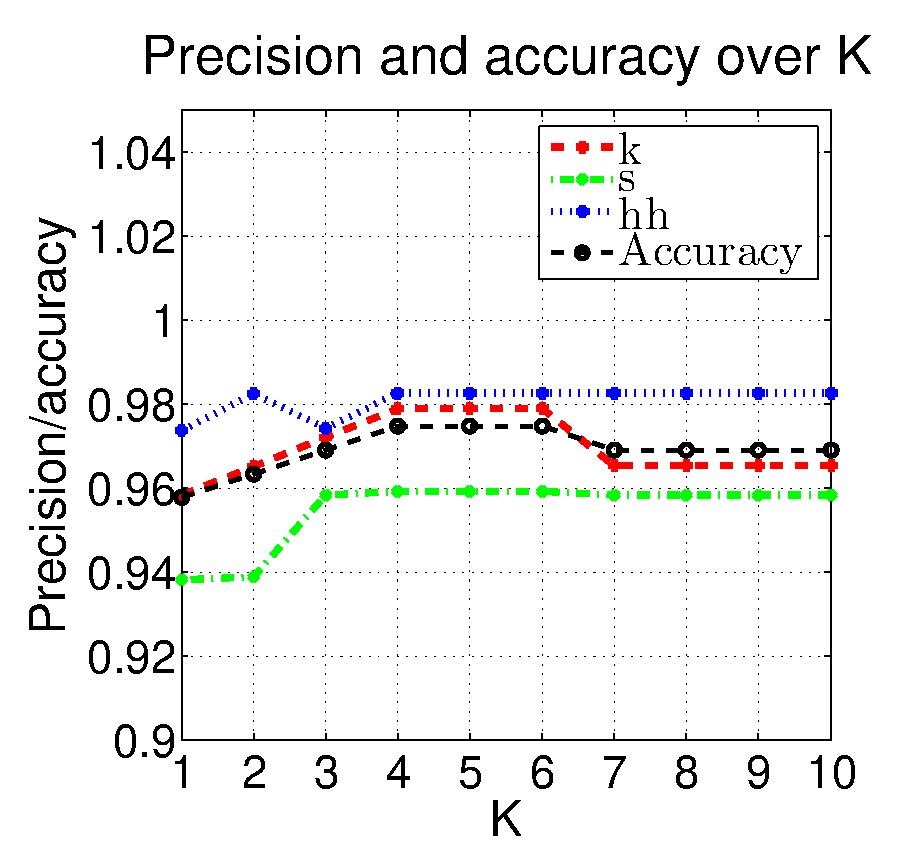
\includegraphics[width=.31\linewidth]{testMFCC10ms5msPrec.eps}}\quad
				\subcaptionbox{Recall}{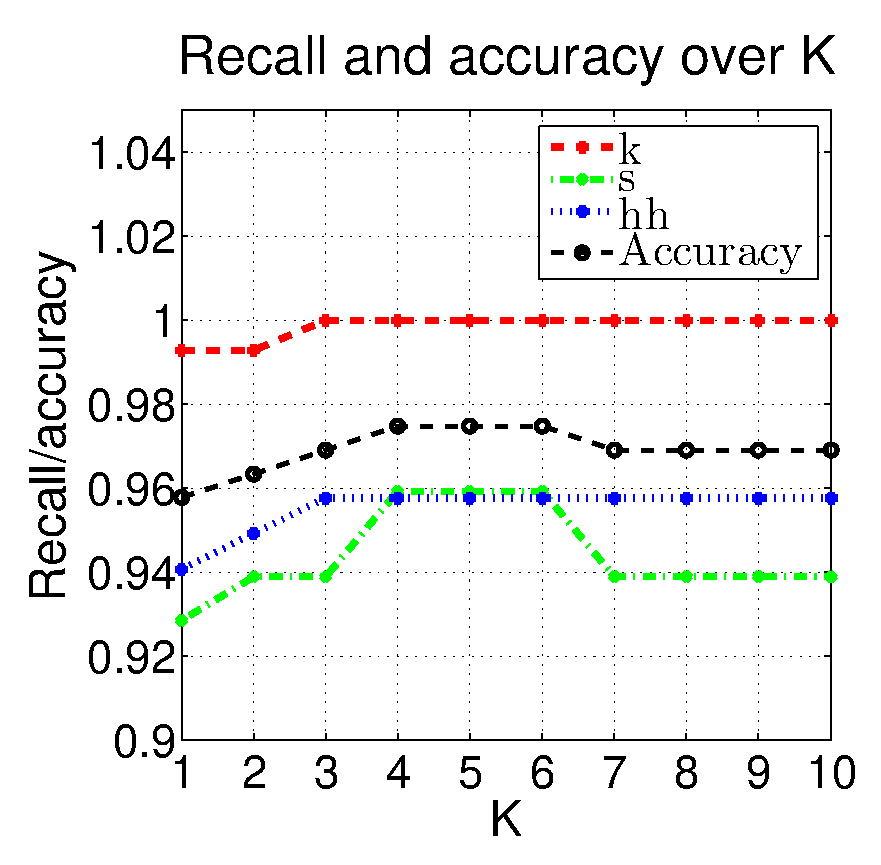
\includegraphics[width=.31\linewidth]{testMFCC10ms5msRec.eps}}\quad
				\subcaptionbox{F}{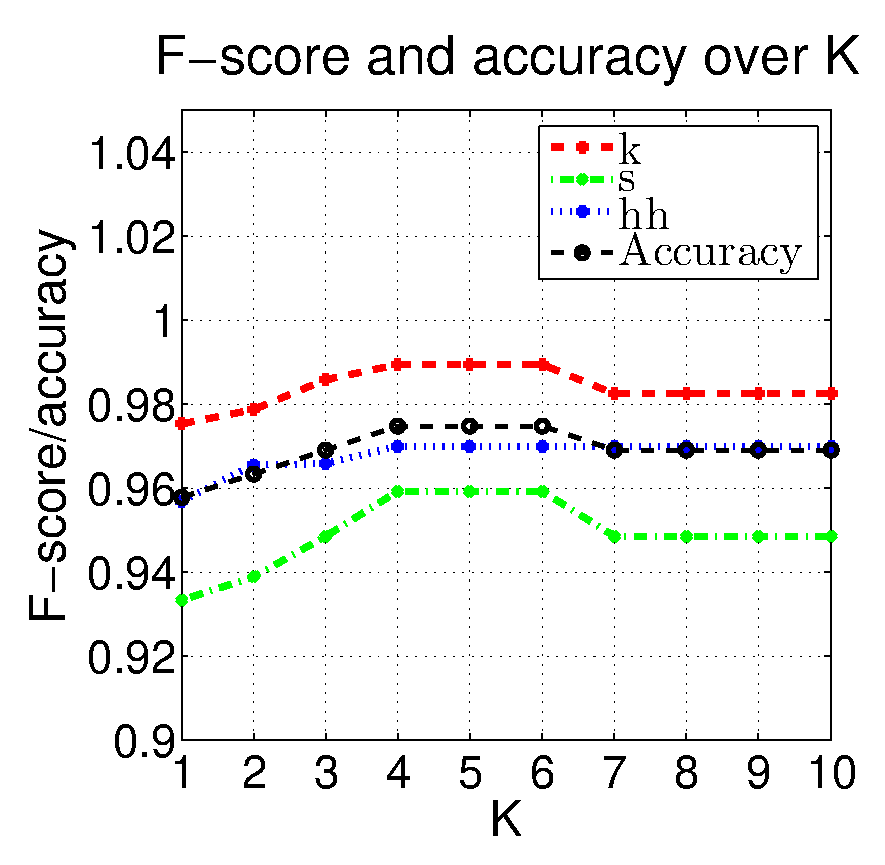
\includegraphics[width=.31\linewidth]{testMFCC10ms5msF.eps}}\quad
				\caption{Result plots for MFCC with 10ms window size and 5ms window skip.}
				\label{fig:eval:testPlotMFCC10ms5ms}
			\end{minipage}\hfill
			
			\begin{minipage}{\textwidth}
				\centering
				\subcaptionbox{Precision}{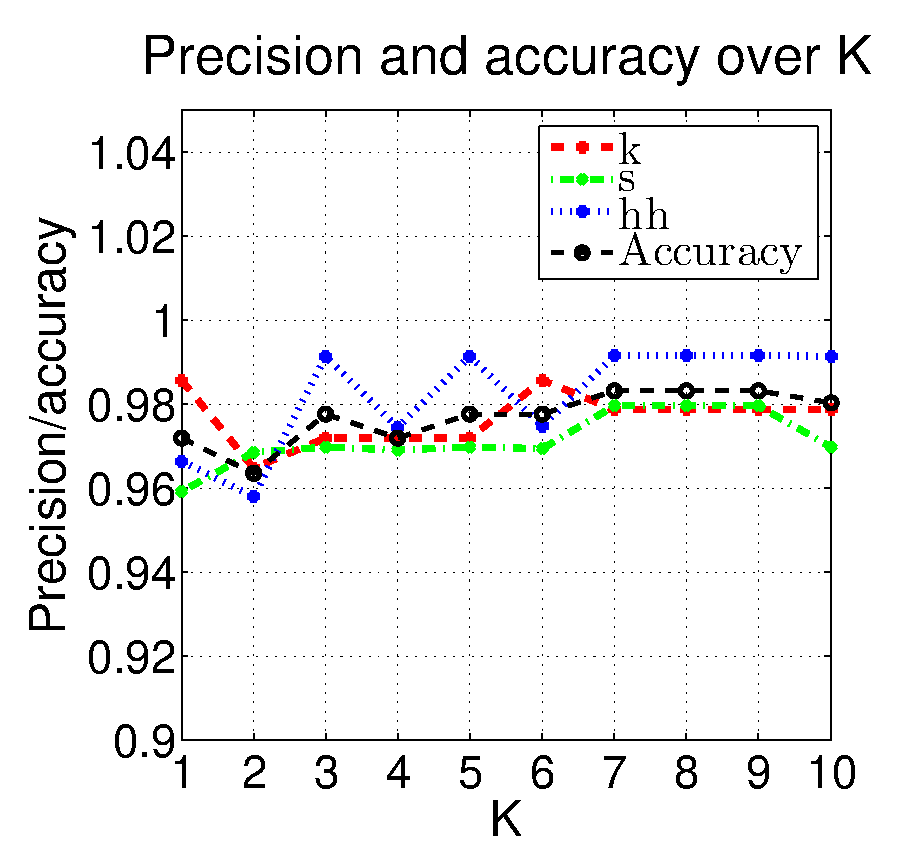
\includegraphics[width=.31\linewidth]{testMFCC5ms2msPrec.eps}}\quad
				\subcaptionbox{Recall}{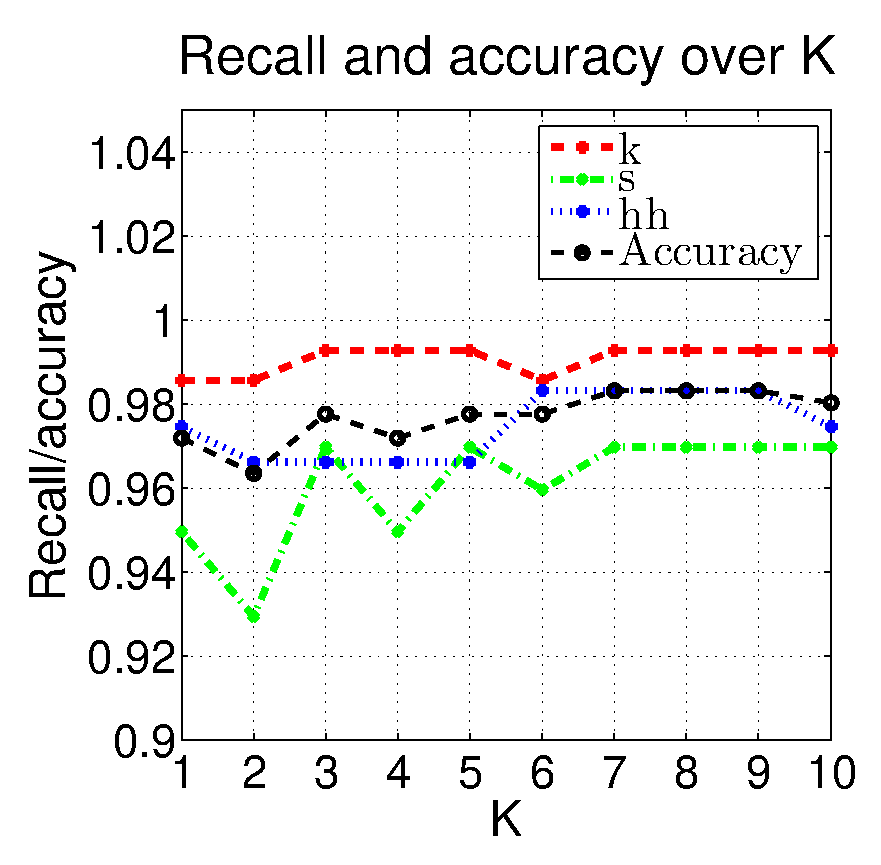
\includegraphics[width=.31\linewidth]{testMFCC5ms2msRec.eps}}\quad
				\subcaptionbox{F}{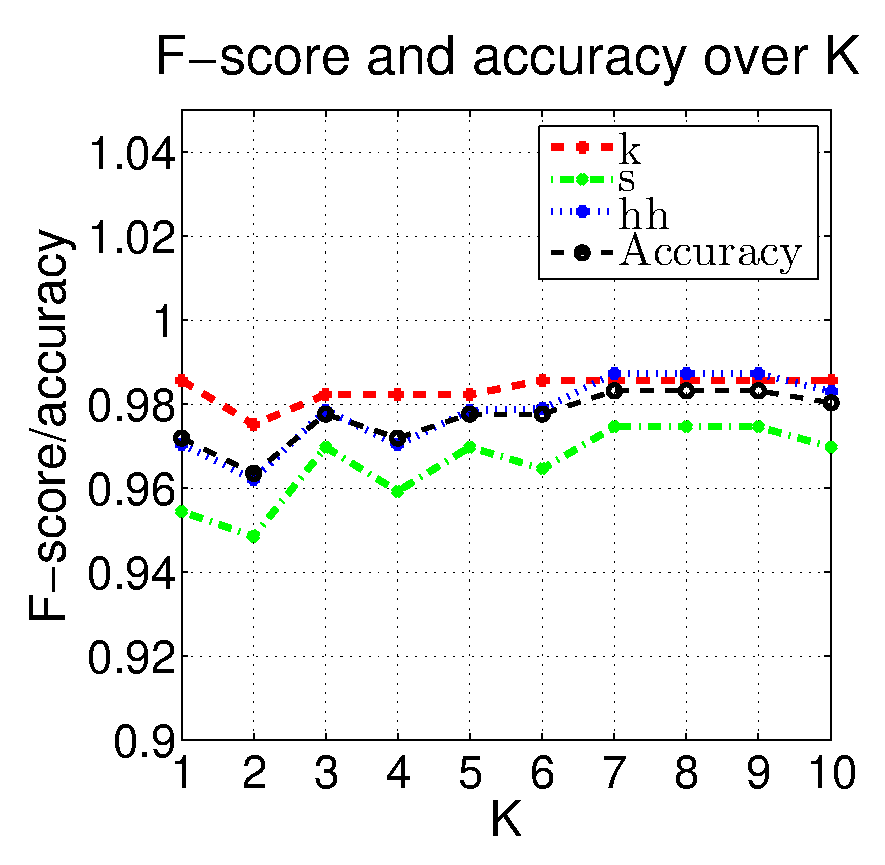
\includegraphics[width=.31\linewidth]{testMFCC5ms2msF.eps}}\quad
				\caption{Result plots for MFCC with 5ms window size and 2ms window skip.}
				\label{fig:eval:testPlotMFCC5ms2ms}
			\end{minipage}\hfill
		\end{figure}
		
		Three different configurations of of the MFCC feature have been tested for $K \in [1;10]$: 20ms,10ms, and 5ms window sizes with 10ms, 5ms, and 2ms window skip respectively. All tests use feature vectors consisting of the first 20 coefficients. 
		
		
		Something about the best/worst case. Include specific confusion tables. Perhaps information specific to each three tests (per feat.), e.g. amount of sounds stripped from each class or similar.
		
		God damn $\chi\sup{2}$
		
		
			
		
\newcolumntype{"}{@{\hskip\tabcolsep\vrule width 1pt\hskip\tabcolsep}}
\begin{table}
\begin{subtable}[h]{0.45\textwidth}
\centering
\begin{tabular}{|c|c|c|c"c|}
\cline{2-5}
 \multicolumn{1}{c|}{} & \textbf{k}  & \textbf{s}  & \textbf{hh}  & Prec.\\ \hline
 \textbf{s} & \textcolor{red}{1.000} & 0.032 & 0.009 & 0.972\\ \hline
 \textbf{k} & 0.000 & \textcolor{red}{0.946} & 0.043 & 0.946\\ \hline
 \textbf{hh} & 0.000 & 0.022 & \textcolor{red}{0.949} & 0.982\\ \Xhline{2\arrayrulewidth}
 Rec. & 1.000 & 0.946 & 0.949 & \multicolumn{1}{c}{\textcolor{blue}{Acc:}}\\ \cline{1-4}
 F & 0.986 & 0.946 & 0.965 & \multicolumn{1}{c}{\textcolor{blue}{0.968}}\\ \cline{1-4}
\end{tabular}
\caption{$K=1$}
\end{subtable}
\hfill
\begin{subtable}[h]{0.45\textwidth}
\centering
\begin{tabular}{|c|c|c|c"c|}
\cline{2-5}
 \multicolumn{1}{c|}{} & \textbf{k}  & \textbf{s}  & \textbf{hh}  & Prec.\\ \hline
 \textbf{s} & \textcolor{red}{1.000} & 0.065 & 0.009 & 0.952\\ \hline
 \textbf{k} & 0.000 & \textcolor{red}{0.925} & 0.051 & 0.935\\ \hline
 \textbf{hh} & 0.000 & 0.011 & \textcolor{red}{0.940} & 0.991\\ \Xhline{2\arrayrulewidth}
 Rec. & 1.000 & 0.925 & 0.940 & \multicolumn{1}{c}{\textcolor{blue}{Acc:}}\\ \cline{1-4}
 F & 0.975 & 0.930 & 0.965 & \multicolumn{1}{c}{\textcolor{blue}{0.960}}\\ \cline{1-4}
\end{tabular}
\caption{$K=2$}
\end{subtable}
\hfill
\begin{subtable}[h]{0.45\textwidth}
\centering
\begin{tabular}{|c|c|c|c"c|}
\cline{2-5}
 \multicolumn{1}{c|}{} & \textbf{k}  & \textbf{s}  & \textbf{hh}  & Prec.\\ \hline
 \textbf{s} & \textcolor{red}{1.000} & 0.022 & 0.000 & 0.986\\ \hline
 \textbf{k} & 0.000 & \textcolor{red}{0.968} & 0.017 & 0.978\\ \hline
 \textbf{hh} & 0.000 & 0.011 & \textcolor{red}{0.983} & 0.991\\ \Xhline{2\arrayrulewidth}
 Rec. & 1.000 & 0.968 & 0.983 & \multicolumn{1}{c}{\textcolor{blue}{Acc:}}\\ \cline{1-4}
 F & 0.993 & 0.973 & 0.987 & \multicolumn{1}{c}{\textcolor{blue}{0.986}}\\ \cline{1-4}
\end{tabular}
\caption{$K=3$}
\end{subtable}
\hfill
\begin{subtable}[h]{0.45\textwidth}
\centering
\begin{tabular}{|c|c|c|c"c|}
\cline{2-5}
 \multicolumn{1}{c|}{} & \textbf{k}  & \textbf{s}  & \textbf{hh}  & Prec.\\ \hline
 \textbf{s} & \textcolor{red}{1.000} & 0.022 & 0.000 & 0.986\\ \hline
 \textbf{k} & 0.000 & \textcolor{red}{0.968} & 0.034 & 0.957\\ \hline
 \textbf{hh} & 0.000 & 0.011 & \textcolor{red}{0.966} & 0.991\\ \Xhline{2\arrayrulewidth}
 Rec. & 1.000 & 0.968 & 0.966 & \multicolumn{1}{c}{\textcolor{blue}{Acc:}}\\ \cline{1-4}
 F & 0.993 & 0.963 & 0.978 & \multicolumn{1}{c}{\textcolor{blue}{0.980}}\\ \cline{1-4}
\end{tabular}
\caption{$K=4$}
\end{subtable}
\hfill
\begin{subtable}[h]{0.45\textwidth}
\centering
\begin{tabular}{|c|c|c|c"c|}
\cline{2-5}
 \multicolumn{1}{c|}{} & \textbf{k}  & \textbf{s}  & \textbf{hh}  & Prec.\\ \hline
 \textbf{s} & \textcolor{red}{1.000} & 0.022 & 0.000 & 0.986\\ \hline
 \textbf{k} & 0.000 & \textcolor{red}{0.957} & 0.009 & 0.989\\ \hline
 \textbf{hh} & 0.000 & 0.022 & \textcolor{red}{0.991} & 0.983\\ \Xhline{2\arrayrulewidth}
 Rec. & 1.000 & 0.957 & 0.991 & \multicolumn{1}{c}{\textcolor{blue}{Acc:}}\\ \cline{1-4}
 F & 0.993 & 0.973 & 0.987 & \multicolumn{1}{c}{\textcolor{blue}{0.986}}\\ \cline{1-4}
\end{tabular}
\caption{$K=5$}
\end{subtable}
\hfill
\begin{subtable}[h]{0.45\textwidth}
\centering
\begin{tabular}{|c|c|c|c"c|}
\cline{2-5}
 \multicolumn{1}{c|}{} & \textbf{k}  & \textbf{s}  & \textbf{hh}  & Prec.\\ \hline
 \textbf{s} & \textcolor{red}{1.000} & 0.022 & 0.000 & 0.986\\ \hline
 \textbf{k} & 0.000 & \textcolor{red}{0.957} & 0.009 & 0.989\\ \hline
 \textbf{hh} & 0.000 & 0.022 & \textcolor{red}{0.991} & 0.983\\ \Xhline{2\arrayrulewidth}
 Rec. & 1.000 & 0.957 & 0.991 & \multicolumn{1}{c}{\textcolor{blue}{Acc:}}\\ \cline{1-4}
 F & 0.993 & 0.973 & 0.987 & \multicolumn{1}{c}{\textcolor{blue}{0.986}}\\ \cline{1-4}
\end{tabular}
\caption{$K=6$}
\end{subtable}
\hfill
\begin{subtable}[h]{0.45\textwidth}
\centering
\begin{tabular}{|c|c|c|c"c|}
\cline{2-5}
 \multicolumn{1}{c|}{} & \textbf{k}  & \textbf{s}  & \textbf{hh}  & Prec.\\ \hline
 \textbf{s} & \textcolor{red}{1.000} & 0.022 & 0.000 & 0.986\\ \hline
 \textbf{k} & 0.000 & \textcolor{red}{0.957} & 0.009 & 0.989\\ \hline
 \textbf{hh} & 0.000 & 0.022 & \textcolor{red}{0.991} & 0.983\\ \Xhline{2\arrayrulewidth}
 Rec. & 1.000 & 0.957 & 0.991 & \multicolumn{1}{c}{\textcolor{blue}{Acc:}}\\ \cline{1-4}
 F & 0.993 & 0.973 & 0.987 & \multicolumn{1}{c}{\textcolor{blue}{0.986}}\\ \cline{1-4}
\end{tabular}
\caption{$K=7$}
\end{subtable}
\hfill
\begin{subtable}[h]{0.45\textwidth}
\centering
\begin{tabular}{|c|c|c|c"c|}
\cline{2-5}
 \multicolumn{1}{c|}{} & \textbf{k}  & \textbf{s}  & \textbf{hh}  & Prec.\\ \hline
 \textbf{s} & \textcolor{red}{1.000} & 0.022 & 0.000 & 0.986\\ \hline
 \textbf{k} & 0.000 & \textcolor{red}{0.957} & 0.009 & 0.989\\ \hline
 \textbf{hh} & 0.000 & 0.022 & \textcolor{red}{0.991} & 0.983\\ \Xhline{2\arrayrulewidth}
 Rec. & 1.000 & 0.957 & 0.991 & \multicolumn{1}{c}{\textcolor{blue}{Acc:}}\\ \cline{1-4}
 F & 0.993 & 0.973 & 0.987 & \multicolumn{1}{c}{\textcolor{blue}{0.986}}\\ \cline{1-4}
\end{tabular}
\caption{$K=8$}
\end{subtable}
\hfill
\begin{subtable}[h]{0.45\textwidth}
\centering
\begin{tabular}{|c|c|c|c"c|}
\cline{2-5}
 \multicolumn{1}{c|}{} & \textbf{k}  & \textbf{s}  & \textbf{hh}  & Prec.\\ \hline
 \textbf{s} & \textcolor{red}{1.000} & 0.022 & 0.009 & 0.979\\ \hline
 \textbf{k} & 0.000 & \textcolor{red}{0.968} & 0.009 & 0.989\\ \hline
 \textbf{hh} & 0.000 & 0.011 & \textcolor{red}{0.983} & 0.991\\ \Xhline{2\arrayrulewidth}
 Rec. & 1.000 & 0.968 & 0.983 & \multicolumn{1}{c}{\textcolor{blue}{Acc:}}\\ \cline{1-4}
 F & 0.989 & 0.978 & 0.987 & \multicolumn{1}{c}{\textcolor{blue}{0.986}}\\ \cline{1-4}
\end{tabular}
\caption{$K=9$}
\end{subtable}
\hfill
\begin{subtable}[h]{0.45\textwidth}
\centering
\begin{tabular}{|c|c|c|c"c|}
\cline{2-5}
 \multicolumn{1}{c|}{} & \textbf{k}  & \textbf{s}  & \textbf{hh}  & Prec.\\ \hline
 \textbf{s} & \textcolor{red}{1.000} & 0.022 & 0.000 & 0.986\\ \hline
 \textbf{k} & 0.000 & \textcolor{red}{0.968} & 0.009 & 0.989\\ \hline
 \textbf{hh} & 0.000 & 0.011 & \textcolor{red}{0.991} & 0.991\\ \Xhline{2\arrayrulewidth}
 Rec. & 1.000 & 0.968 & 0.991 & \multicolumn{1}{c}{\textcolor{blue}{Acc:}}\\ \cline{1-4}
 F & 0.993 & 0.978 & 0.991 & \multicolumn{1}{c}{\textcolor{blue}{0.989}}\\ \cline{1-4}
\end{tabular}
\caption{$K=10$}
\end{subtable}
\hfill

\caption{Confusion tables for MFCC feature vectors using 20ms window size and 10ms window skip.}
\label{table:eval:mfcc20ms10ms}

\end{table}
		\newcolumntype{"}{@{\hskip\tabcolsep\vrule width 1pt\hskip\tabcolsep}}
\begin{table}
\begin{subtable}[h]{0.45\textwidth}
\centering
\begin{tabular}{|c|c|c|c"c|}
\cline{2-5}
 \multicolumn{1}{c|}{} & \textbf{k}  & \textbf{s}  & \textbf{hh}  & Prec.\\ \hline
 \textbf{s} & \textcolor{red}{0.993} & 0.041 & 0.017 & 0.958\\ \hline
 \textbf{k} & 0.007 & \textcolor{red}{0.929} & 0.042 & 0.938\\ \hline
 \textbf{hh} & 0.007 & 0.031 & \textcolor{red}{0.941} & 0.974\\ \Xhline{2\arrayrulewidth}
 Rec. & 0.993 & 0.929 & 0.941 & \multicolumn{1}{c}{\textcolor{blue}{Acc:}}\\ \cline{1-4}
 F & 0.975 & 0.933 & 0.957 & \multicolumn{1}{c}{\textcolor{blue}{0.958}}\\ \cline{1-4}
\end{tabular}
\caption{$K=1$}
\end{subtable}
\hfill
\begin{subtable}[h]{0.45\textwidth}
\centering
\begin{tabular}{|c|c|c|c"c|}
\cline{2-5}
 \multicolumn{1}{c|}{} & \textbf{k}  & \textbf{s}  & \textbf{hh}  & Prec.\\ \hline
 \textbf{s} & \textcolor{red}{0.993} & 0.041 & 0.008 & 0.965\\ \hline
 \textbf{k} & 0.007 & \textcolor{red}{0.939} & 0.042 & 0.939\\ \hline
 \textbf{hh} & 0.007 & 0.020 & \textcolor{red}{0.949} & 0.982\\ \Xhline{2\arrayrulewidth}
 Rec. & 0.993 & 0.939 & 0.949 & \multicolumn{1}{c}{\textcolor{blue}{Acc:}}\\ \cline{1-4}
 F & 0.979 & 0.939 & 0.966 & \multicolumn{1}{c}{\textcolor{blue}{0.963}}\\ \cline{1-4}
\end{tabular}
\caption{$K=2$}
\end{subtable}
\hfill
\begin{subtable}[h]{0.45\textwidth}
\centering
\begin{tabular}{|c|c|c|c"c|}
\cline{2-5}
 \multicolumn{1}{c|}{} & \textbf{k}  & \textbf{s}  & \textbf{hh}  & Prec.\\ \hline
 \textbf{s} & \textcolor{red}{1.000} & 0.031 & 0.008 & 0.972\\ \hline
 \textbf{k} & 0.000 & \textcolor{red}{0.939} & 0.034 & 0.958\\ \hline
 \textbf{hh} & 0.000 & 0.031 & \textcolor{red}{0.958} & 0.974\\ \Xhline{2\arrayrulewidth}
 Rec. & 1.000 & 0.939 & 0.958 & \multicolumn{1}{c}{\textcolor{blue}{Acc:}}\\ \cline{1-4}
 F & 0.986 & 0.948 & 0.966 & \multicolumn{1}{c}{\textcolor{blue}{0.969}}\\ \cline{1-4}
\end{tabular}
\caption{$K=3$}
\end{subtable}
\hfill
\begin{subtable}[h]{0.45\textwidth}
\centering
\begin{tabular}{|c|c|c|c"c|}
\cline{2-5}
 \multicolumn{1}{c|}{} & \textbf{k}  & \textbf{s}  & \textbf{hh}  & Prec.\\ \hline
 \textbf{s} & \textcolor{red}{1.000} & 0.020 & 0.008 & 0.979\\ \hline
 \textbf{k} & 0.000 & \textcolor{red}{0.959} & 0.034 & 0.959\\ \hline
 \textbf{hh} & 0.000 & 0.020 & \textcolor{red}{0.958} & 0.983\\ \Xhline{2\arrayrulewidth}
 Rec. & 1.000 & 0.959 & 0.958 & \multicolumn{1}{c}{\textcolor{blue}{Acc:}}\\ \cline{1-4}
 F & 0.989 & 0.959 & 0.970 & \multicolumn{1}{c}{\textcolor{blue}{0.975}}\\ \cline{1-4}
\end{tabular}
\caption{$K=4$}
\end{subtable}
\hfill
\begin{subtable}[h]{0.45\textwidth}
\centering
\begin{tabular}{|c|c|c|c"c|}
\cline{2-5}
 \multicolumn{1}{c|}{} & \textbf{k}  & \textbf{s}  & \textbf{hh}  & Prec.\\ \hline
 \textbf{s} & \textcolor{red}{1.000} & 0.020 & 0.008 & 0.979\\ \hline
 \textbf{k} & 0.000 & \textcolor{red}{0.959} & 0.034 & 0.959\\ \hline
 \textbf{hh} & 0.000 & 0.020 & \textcolor{red}{0.958} & 0.983\\ \Xhline{2\arrayrulewidth}
 Rec. & 1.000 & 0.959 & 0.958 & \multicolumn{1}{c}{\textcolor{blue}{Acc:}}\\ \cline{1-4}
 F & 0.989 & 0.959 & 0.970 & \multicolumn{1}{c}{\textcolor{blue}{0.975}}\\ \cline{1-4}
\end{tabular}
\caption{$K=5$}
\end{subtable}
\hfill
\begin{subtable}[h]{0.45\textwidth}
\centering
\begin{tabular}{|c|c|c|c"c|}
\cline{2-5}
 \multicolumn{1}{c|}{} & \textbf{k}  & \textbf{s}  & \textbf{hh}  & Prec.\\ \hline
 \textbf{s} & \textcolor{red}{1.000} & 0.020 & 0.008 & 0.979\\ \hline
 \textbf{k} & 0.000 & \textcolor{red}{0.959} & 0.034 & 0.959\\ \hline
 \textbf{hh} & 0.000 & 0.020 & \textcolor{red}{0.958} & 0.983\\ \Xhline{2\arrayrulewidth}
 Rec. & 1.000 & 0.959 & 0.958 & \multicolumn{1}{c}{\textcolor{blue}{Acc:}}\\ \cline{1-4}
 F & 0.989 & 0.959 & 0.970 & \multicolumn{1}{c}{\textcolor{blue}{0.975}}\\ \cline{1-4}
\end{tabular}
\caption{$K=6$}
\end{subtable}
\hfill
\begin{subtable}[h]{0.45\textwidth}
\centering
\begin{tabular}{|c|c|c|c"c|}
\cline{2-5}
 \multicolumn{1}{c|}{} & \textbf{k}  & \textbf{s}  & \textbf{hh}  & Prec.\\ \hline
 \textbf{s} & \textcolor{red}{1.000} & 0.041 & 0.008 & 0.965\\ \hline
 \textbf{k} & 0.000 & \textcolor{red}{0.939} & 0.034 & 0.958\\ \hline
 \textbf{hh} & 0.000 & 0.020 & \textcolor{red}{0.958} & 0.983\\ \Xhline{2\arrayrulewidth}
 Rec. & 1.000 & 0.939 & 0.958 & \multicolumn{1}{c}{\textcolor{blue}{Acc:}}\\ \cline{1-4}
 F & 0.982 & 0.948 & 0.970 & \multicolumn{1}{c}{\textcolor{blue}{0.969}}\\ \cline{1-4}
\end{tabular}
\caption{$K=7$}
\end{subtable}
\hfill
\begin{subtable}[h]{0.45\textwidth}
\centering
\begin{tabular}{|c|c|c|c"c|}
\cline{2-5}
 \multicolumn{1}{c|}{} & \textbf{k}  & \textbf{s}  & \textbf{hh}  & Prec.\\ \hline
 \textbf{s} & \textcolor{red}{1.000} & 0.041 & 0.008 & 0.965\\ \hline
 \textbf{k} & 0.000 & \textcolor{red}{0.939} & 0.034 & 0.958\\ \hline
 \textbf{hh} & 0.000 & 0.020 & \textcolor{red}{0.958} & 0.983\\ \Xhline{2\arrayrulewidth}
 Rec. & 1.000 & 0.939 & 0.958 & \multicolumn{1}{c}{\textcolor{blue}{Acc:}}\\ \cline{1-4}
 F & 0.982 & 0.948 & 0.970 & \multicolumn{1}{c}{\textcolor{blue}{0.969}}\\ \cline{1-4}
\end{tabular}
\caption{$K=8$}
\end{subtable}
\hfill
\begin{subtable}[h]{0.45\textwidth}
\centering
\begin{tabular}{|c|c|c|c"c|}
\cline{2-5}
 \multicolumn{1}{c|}{} & \textbf{k}  & \textbf{s}  & \textbf{hh}  & Prec.\\ \hline
 \textbf{s} & \textcolor{red}{1.000} & 0.041 & 0.008 & 0.965\\ \hline
 \textbf{k} & 0.000 & \textcolor{red}{0.939} & 0.034 & 0.958\\ \hline
 \textbf{hh} & 0.000 & 0.020 & \textcolor{red}{0.958} & 0.983\\ \Xhline{2\arrayrulewidth}
 Rec. & 1.000 & 0.939 & 0.958 & \multicolumn{1}{c}{\textcolor{blue}{Acc:}}\\ \cline{1-4}
 F & 0.982 & 0.948 & 0.970 & \multicolumn{1}{c}{\textcolor{blue}{0.969}}\\ \cline{1-4}
\end{tabular}
\caption{$K=9$}
\end{subtable}
\hfill
\begin{subtable}[h]{0.45\textwidth}
\centering
\begin{tabular}{|c|c|c|c"c|}
\cline{2-5}
 \multicolumn{1}{c|}{} & \textbf{k}  & \textbf{s}  & \textbf{hh}  & Prec.\\ \hline
 \textbf{s} & \textcolor{red}{1.000} & 0.041 & 0.008 & 0.965\\ \hline
 \textbf{k} & 0.000 & \textcolor{red}{0.939} & 0.034 & 0.958\\ \hline
 \textbf{hh} & 0.000 & 0.020 & \textcolor{red}{0.958} & 0.983\\ \Xhline{2\arrayrulewidth}
 Rec. & 1.000 & 0.939 & 0.958 & \multicolumn{1}{c}{\textcolor{blue}{Acc:}}\\ \cline{1-4}
 F & 0.982 & 0.948 & 0.970 & \multicolumn{1}{c}{\textcolor{blue}{0.969}}\\ \cline{1-4}
\end{tabular}
\caption{$K=10$}
\end{subtable}
\hfill

\caption{Confusion tables for MFCC feature vectors using 20ms window size and 10ms window skip.}
\label{table:eval:mfcc20ms10ms}

\end{table}
		
\newcolumntype{"}{@{\hskip\tabcolsep\vrule width 1pt\hskip\tabcolsep}}
\begin{table}
\begin{subtable}[h]{0.45\textwidth}
\centering
\begin{tabular}{|c|c|c|c"c|}
\cline{2-5}
 \multicolumn{1}{c|}{} & \textbf{k}  & \textbf{s}  & \textbf{hh}  & Prec.\\ \hline
 \textbf{s} & \textcolor{red}{0.986} & 0.020 & 0.000 & 0.986\\ \hline
 \textbf{k} & 0.007 & \textcolor{red}{0.949} & 0.025 & 0.959\\ \hline
 \textbf{hh} & 0.007 & 0.030 & \textcolor{red}{0.975} & 0.966\\ \Xhline{2\arrayrulewidth}
 Rec. & 0.986 & 0.949 & 0.975 & \multicolumn{1}{c}{\textcolor{blue}{Acc:}}\\ \cline{1-4}
 F & 0.986 & 0.954 & 0.970 & \multicolumn{1}{c}{\textcolor{blue}{0.972}}\\ \cline{1-4}
\end{tabular}
\caption{$K=1$}
\end{subtable}
\hfill
\begin{subtable}[h]{0.45\textwidth}
\centering
\begin{tabular}{|c|c|c|c"c|}
\cline{2-5}
 \multicolumn{1}{c|}{} & \textbf{k}  & \textbf{s}  & \textbf{hh}  & Prec.\\ \hline
 \textbf{s} & \textcolor{red}{0.986} & 0.030 & 0.017 & 0.965\\ \hline
 \textbf{k} & 0.007 & \textcolor{red}{0.929} & 0.017 & 0.968\\ \hline
 \textbf{hh} & 0.007 & 0.040 & \textcolor{red}{0.966} & 0.958\\ \Xhline{2\arrayrulewidth}
 Rec. & 0.986 & 0.929 & 0.966 & \multicolumn{1}{c}{\textcolor{blue}{Acc:}}\\ \cline{1-4}
 F & 0.975 & 0.948 & 0.962 & \multicolumn{1}{c}{\textcolor{blue}{0.963}}\\ \cline{1-4}
\end{tabular}
\caption{$K=2$}
\end{subtable}
\hfill
\begin{subtable}[h]{0.45\textwidth}
\centering
\begin{tabular}{|c|c|c|c"c|}
\cline{2-5}
 \multicolumn{1}{c|}{} & \textbf{k}  & \textbf{s}  & \textbf{hh}  & Prec.\\ \hline
 \textbf{s} & \textcolor{red}{0.993} & 0.020 & 0.017 & 0.972\\ \hline
 \textbf{k} & 0.007 & \textcolor{red}{0.970} & 0.017 & 0.970\\ \hline
 \textbf{hh} & 0.007 & 0.010 & \textcolor{red}{0.966} & 0.991\\ \Xhline{2\arrayrulewidth}
 Rec. & 0.993 & 0.970 & 0.966 & \multicolumn{1}{c}{\textcolor{blue}{Acc:}}\\ \cline{1-4}
 F & 0.982 & 0.970 & 0.979 & \multicolumn{1}{c}{\textcolor{blue}{0.978}}\\ \cline{1-4}
\end{tabular}
\caption{$K=3$}
\end{subtable}
\hfill
\begin{subtable}[h]{0.45\textwidth}
\centering
\begin{tabular}{|c|c|c|c"c|}
\cline{2-5}
 \multicolumn{1}{c|}{} & \textbf{k}  & \textbf{s}  & \textbf{hh}  & Prec.\\ \hline
 \textbf{s} & \textcolor{red}{0.993} & 0.020 & 0.017 & 0.972\\ \hline
 \textbf{k} & 0.007 & \textcolor{red}{0.949} & 0.017 & 0.969\\ \hline
 \textbf{hh} & 0.007 & 0.030 & \textcolor{red}{0.966} & 0.974\\ \Xhline{2\arrayrulewidth}
 Rec. & 0.993 & 0.949 & 0.966 & \multicolumn{1}{c}{\textcolor{blue}{Acc:}}\\ \cline{1-4}
 F & 0.982 & 0.959 & 0.970 & \multicolumn{1}{c}{\textcolor{blue}{0.972}}\\ \cline{1-4}
\end{tabular}
\caption{$K=4$}
\end{subtable}
\hfill
\begin{subtable}[h]{0.45\textwidth}
\centering
\begin{tabular}{|c|c|c|c"c|}
\cline{2-5}
 \multicolumn{1}{c|}{} & \textbf{k}  & \textbf{s}  & \textbf{hh}  & Prec.\\ \hline
 \textbf{s} & \textcolor{red}{0.993} & 0.020 & 0.017 & 0.972\\ \hline
 \textbf{k} & 0.007 & \textcolor{red}{0.970} & 0.017 & 0.970\\ \hline
 \textbf{hh} & 0.007 & 0.010 & \textcolor{red}{0.966} & 0.991\\ \Xhline{2\arrayrulewidth}
 Rec. & 0.993 & 0.970 & 0.966 & \multicolumn{1}{c}{\textcolor{blue}{Acc:}}\\ \cline{1-4}
 F & 0.982 & 0.970 & 0.979 & \multicolumn{1}{c}{\textcolor{blue}{0.978}}\\ \cline{1-4}
\end{tabular}
\caption{$K=5$}
\end{subtable}
\hfill
\begin{subtable}[h]{0.45\textwidth}
\centering
\begin{tabular}{|c|c|c|c"c|}
\cline{2-5}
 \multicolumn{1}{c|}{} & \textbf{k}  & \textbf{s}  & \textbf{hh}  & Prec.\\ \hline
 \textbf{s} & \textcolor{red}{0.986} & 0.020 & 0.000 & 0.986\\ \hline
 \textbf{k} & 0.007 & \textcolor{red}{0.960} & 0.017 & 0.969\\ \hline
 \textbf{hh} & 0.007 & 0.020 & \textcolor{red}{0.983} & 0.975\\ \Xhline{2\arrayrulewidth}
 Rec. & 0.986 & 0.960 & 0.983 & \multicolumn{1}{c}{\textcolor{blue}{Acc:}}\\ \cline{1-4}
 F & 0.986 & 0.964 & 0.979 & \multicolumn{1}{c}{\textcolor{blue}{0.978}}\\ \cline{1-4}
\end{tabular}
\caption{$K=6$}
\end{subtable}
\hfill
\begin{subtable}[h]{0.45\textwidth}
\centering
\begin{tabular}{|c|c|c|c"c|}
\cline{2-5}
 \multicolumn{1}{c|}{} & \textbf{k}  & \textbf{s}  & \textbf{hh}  & Prec.\\ \hline
 \textbf{s} & \textcolor{red}{0.993} & 0.020 & 0.008 & 0.979\\ \hline
 \textbf{k} & 0.007 & \textcolor{red}{0.970} & 0.008 & 0.980\\ \hline
 \textbf{hh} & 0.007 & 0.010 & \textcolor{red}{0.983} & 0.991\\ \Xhline{2\arrayrulewidth}
 Rec. & 0.993 & 0.970 & 0.983 & \multicolumn{1}{c}{\textcolor{blue}{Acc:}}\\ \cline{1-4}
 F & 0.986 & 0.975 & 0.987 & \multicolumn{1}{c}{\textcolor{blue}{0.983}}\\ \cline{1-4}
\end{tabular}
\caption{$K=7$}
\end{subtable}
\hfill
\begin{subtable}[h]{0.45\textwidth}
\centering
\begin{tabular}{|c|c|c|c"c|}
\cline{2-5}
 \multicolumn{1}{c|}{} & \textbf{k}  & \textbf{s}  & \textbf{hh}  & Prec.\\ \hline
 \textbf{s} & \textcolor{red}{0.993} & 0.020 & 0.008 & 0.979\\ \hline
 \textbf{k} & 0.007 & \textcolor{red}{0.970} & 0.008 & 0.980\\ \hline
 \textbf{hh} & 0.007 & 0.010 & \textcolor{red}{0.983} & 0.991\\ \Xhline{2\arrayrulewidth}
 Rec. & 0.993 & 0.970 & 0.983 & \multicolumn{1}{c}{\textcolor{blue}{Acc:}}\\ \cline{1-4}
 F & 0.986 & 0.975 & 0.987 & \multicolumn{1}{c}{\textcolor{blue}{0.983}}\\ \cline{1-4}
\end{tabular}
\caption{$K=8$}
\end{subtable}
\hfill
\begin{subtable}[h]{0.45\textwidth}
\centering
\begin{tabular}{|c|c|c|c"c|}
\cline{2-5}
 \multicolumn{1}{c|}{} & \textbf{k}  & \textbf{s}  & \textbf{hh}  & Prec.\\ \hline
 \textbf{s} & \textcolor{red}{0.993} & 0.020 & 0.008 & 0.979\\ \hline
 \textbf{k} & 0.007 & \textcolor{red}{0.970} & 0.008 & 0.980\\ \hline
 \textbf{hh} & 0.007 & 0.010 & \textcolor{red}{0.983} & 0.991\\ \Xhline{2\arrayrulewidth}
 Rec. & 0.993 & 0.970 & 0.983 & \multicolumn{1}{c}{\textcolor{blue}{Acc:}}\\ \cline{1-4}
 F & 0.986 & 0.975 & 0.987 & \multicolumn{1}{c}{\textcolor{blue}{0.983}}\\ \cline{1-4}
\end{tabular}
\caption{$K=9$}
\end{subtable}
\hfill
\begin{subtable}[h]{0.45\textwidth}
\centering
\begin{tabular}{|c|c|c|c"c|}
\cline{2-5}
 \multicolumn{1}{c|}{} & \textbf{k}  & \textbf{s}  & \textbf{hh}  & Prec.\\ \hline
 \textbf{s} & \textcolor{red}{0.993} & 0.020 & 0.008 & 0.979\\ \hline
 \textbf{k} & 0.007 & \textcolor{red}{0.970} & 0.017 & 0.970\\ \hline
 \textbf{hh} & 0.007 & 0.010 & \textcolor{red}{0.975} & 0.991\\ \Xhline{2\arrayrulewidth}
 Rec. & 0.993 & 0.970 & 0.975 & \multicolumn{1}{c}{\textcolor{blue}{Acc:}}\\ \cline{1-4}
 F & 0.986 & 0.970 & 0.983 & \multicolumn{1}{c}{\textcolor{blue}{0.980}}\\ \cline{1-4}
\end{tabular}
\caption{$K=10$}
\end{subtable}
\hfill

\caption{Confusion tables for MFCC feature vectors using 20ms window size and 10ms window skip.}
\label{table:eval:mfcc20ms10ms}

\end{table}
	
	
	\subsection{Spectral Flux}
		Repeat above procedure for a couple of features, yes, please.